\documentclass[12pt]{article}
\usepackage[a4paper, margin=2cm]{geometry}
\usepackage[english]{babel} % To obtain English text with the blindtext package
\usepackage{blindtext}
\usepackage{graphicx} % Required for inserting images
\usepackage{array, multirow} % For extra column formatting
\usepackage{amsmath, amssymb, cancel} %for equation environment
\usepackage{float}
\usepackage{parskip} % For gaps between para
\usepackage{setspace}
\usepackage{pdfpages}
\usepackage{abstract}
\usepackage[export]{adjustbox}
\usepackage{emptypage}
\usepackage{tocloft}
\usepackage[nottoc]{tocbibind}
\usepackage{hyperref, url}
\usepackage[table]{xcolor}
\usepackage{minted}
    \usemintedstyle{monokai}
\usepackage{caption}
    \captionsetup{font=footnotesize,labelfont=bf}
\usepackage{tcolorbox}
    \newtcolorbox{mintedbox}{
        colback=backcolour,
        boxrule=0pt,
        sharp corners,
        width=\linewidth,
        left=0pt, right=0pt,
        top=3pt, bottom=3pt
    }

\cftsetindents{section}{0em}{2em}
\cftsetindents{subsection}{0em}{2em}

\renewcommand\cfttoctitlefont{\hfill\Large\bfseries}
\renewcommand\cftaftertoctitle{\hfill\mbox{}}

\graphicspath{ {./images/} }

\pagenumbering{arabic}

\definecolor{blurple}{HTML}{5865F2}
\definecolor{backcolour}{HTML}{272823}

\hypersetup{
    colorlinks=true,
    linkcolor=black,
    urlcolor=blurple,
    citecolor=blurple,
}

\urlstyle{same}

\renewcommand{\arraystretch}{1.3}

\setcounter{secnumdepth}{5}
\setcounter{tocdepth}{5}
\newcommand\simpleparagraph[1]{%
  \stepcounter{paragraph}\paragraph*{\theparagraph\quad{}#1}}

%%%%%%%%%%%%%%%%%%%%%%%%%%%%%%%%%%%


\title{PHYC20040 Exp.2 Pleiades SM}
\author{Joana Adao}
\date{\today}

\begin{document}

\begin{titlepage}
    \begin{center}

        \begin{figure}[ht]
            
\includegraphics[width=\textwidth]{UCDLogo.png}
        \end{figure}
        
        \begin{figure}
            \centerline{
\includegraphics[width=\paperwidth]{UCDBanner.png}}
        \end{figure}

        \vspace{4cm}

        {\LARGE \bfseries PHYC20080 Fields, Waves and Light}\\
        \vspace{0.75cm}
        {\Large Experiment No.2 Waves and Resonance}
        
        \vspace{1cm}
    
    {\Large \textbf{18 February 2025}}

    \vspace{2cm}
    
    {\large \textbf{by Joana C.C. Adao (Student No. 23311051)}}\\
    \vspace{.25cm}
    {\large \textbf{With,} Beau Etac}\\
    \vspace{0.25cm}
    {\large Tuesday 16.00-18.00 Slot}\\
    {\large Nicki (Coordinator)}

    \end{center}
    
   \clearpage

\end{titlepage}

\setcounter{page}{1}
\tableofcontents

\newpage

\begin{abstract}
\addcontentsline{toc}{section}{Abstract}

The aim of this experiment was to 

\end{abstract}

%%%%%%%%%%%%%%%%%%%%%%%%%%%%%%%%%%%

\section{Theory} \label{sec:1}


\subsection{Waves}

There are two types of mechanical waves, as illustrated in figure \ref{fig:wavetype}, \textbf{transverse} and \textbf{longitudinal}.

\begin{minipage}{.47\textwidth}
    \captionsetup{hypcap=false}
    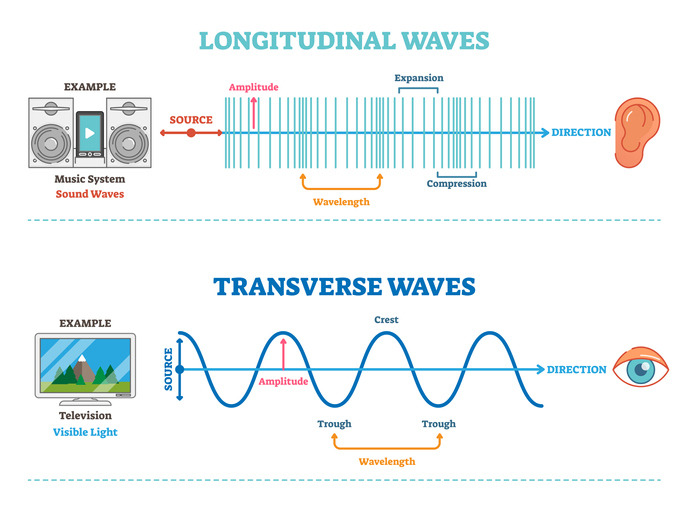
\includegraphics[width=\linewidth]{wavetype.jpg}
    \captionof{figure}{\centering Types of waves \protect\cite{waveoer}.}
    \label{fig:wavetype}
\end{minipage}
\hfill
\begin{minipage}{.51\textwidth}
    \captionsetup{hypcap=false}
    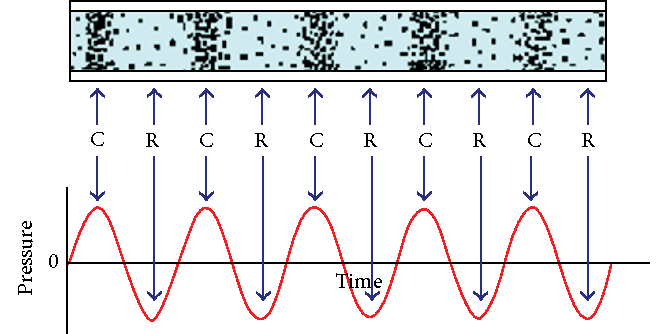
\includegraphics[width=\linewidth]{longtrans.png}
    \captionof{figure}{\centering Longitudinal wave graphed as a transverse wave \protect\cite{mungwave}.}
    \label{fig:longtrans}
\end{minipage}

\textbf{Transverse waves} travel in a series of peaks and troughs with \textit{perpendicular} vibration to the motion. These are the kinds of waves seen when water ripples \cite{waveffden}.
\textbf{Longitudinal waves} vibrate \textit{parallel} to the motion. Instead of peaks and troughs there are areas of compression, in which the molecules around it bunch together, and
areas of rarefraction, in which the molecules are pulled away and space out \cite{waveffden,studywave,acousticsound}.
Through graphing, a longitudinal wave can appear as a transverse wave where the peaks represent compression and troughs represent rarefraction (see figure \ref{fig:longtrans}).

\subsubsection{The Anatomy of a Wave}

There are 4 basic components to a wave \cite{wavebyju,waveffden}, with all components illustrated in figure \ref{fig:waveprop}:

\begin{itemize}
    \item \textbf{Frequency (f):} the number of waves that pass by a point per second (repetitions).
    \item \textbf{Period (T):} time taken for a wave to pass a specific point in a second.
    \item \textbf{Wavelength ($\mathbf{\lambda}$):} the distance between two waves, crest (peak) to crest or trough (valley) to trough.
    \item \textbf{Amplitude (A):} the 'height' of the wave measured from the middle (x-axis) of the wave to the crest/trough.
\end{itemize}

\begin{figure}[H]
    \centering
    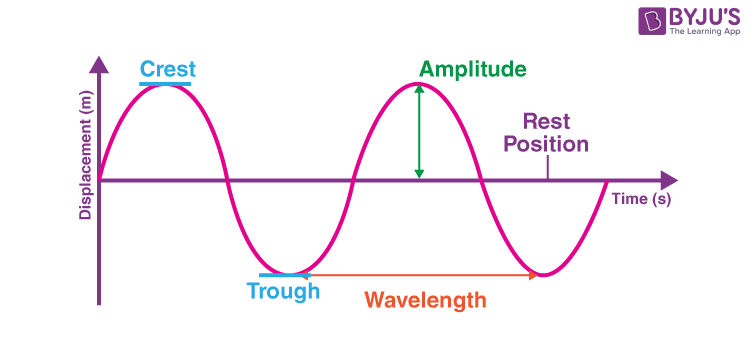
\includegraphics[width=14cm]{wave.png}
    \caption{\centering Features of a wave \protect\cite{wavebyju}}
    \label{fig:waveprop}
\end{figure}


\subsubsection{Newton's Laws and Wave Velocity}

The velocity of a wave can be found at a specific point on a waveform (a point of fixed phase) by relating the wavelength to the period/frequency \cite{geekwave,librewave}:

\vspace{-1.5ex}
\begin{gather} \label{eq:1}
    v = \frac{\lambda}{T} = \lambda f
\end{gather}

Furthermore, by applying Newton's second law to the vertical direction of the wave the following is able to be derived \cite{librewave}:

\vspace{-1.5ex}
\begin{gather} \label{eq:2}
    v = \sqrt{\frac{\textbf{F}}{\mu}} = \sqrt{\frac{T}{\mu}}
\end{gather}

Where \textbf{F} is a force acting on the wave, pulling through the string. This can be defined as the tension \textbf{T}, the force of a stretched material (eg. string). $\mathbf{\mu}$ is then
the mass per unit length of the string.

\subsection{Resonance}

Resonance is a phenomenon in which an object will vibrate more strongly when an external oscillation that matches its own natural frequency passes through it \cite{resbrit,reslibre}.

Equation \ref{eq:1} and equation \ref{eq:1} can be combined to give the following:

\vspace{-1.5ex}
\begin{gather} \label{eq:3}
    \lambda f = \sqrt{\frac{T}{\mu}} \quad \implies \quad f = \frac{1}{\lambda} \sqrt{\frac{T}{\mu}}
\end{gather}

\subsubsection{Standing Waves} \label{sec:1.2.1}

Standing waves are produced as a result of interference from the \textit{reflected wave} when a wave encounters a boundary between two mediums \cite{librestand,MARION1981341,OZEROV2007105,isaacwave}.
There appears to be a point along the axis of the wave which is fixed and the wave oscillates on, known as \textit{nodes}. The rest of the wave that moves to the crests and troughs are known as \textit{antinodes}
\cite{isaacwave}.
The resulting wave is a superposition of the adjacent nodes and antinodes that are, naturally, in phase \cite{isaacwave,librestand,MARION1981341}.

\begin{figure}[H]
    \centering
    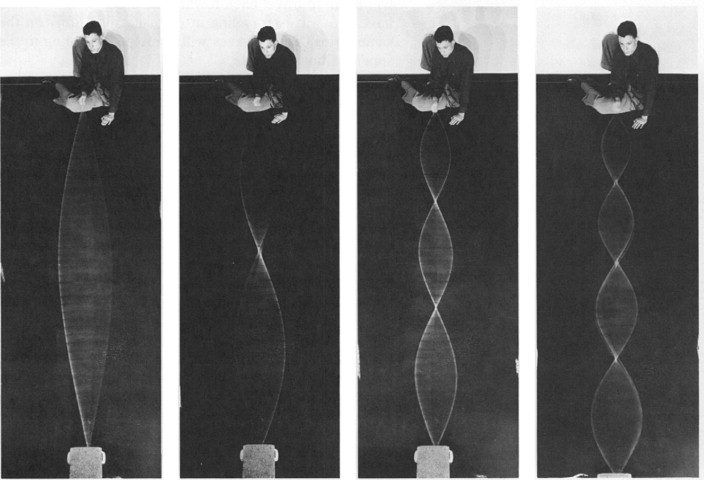
\includegraphics[width=10cm]{standing waves.jpg}
    \caption{\centering Standing waves in a stretched rubber tube \protect\cite{MARION1981341}.}
    \label{fig:stand}
\end{figure}

The lowest frequency at which a standing wave only produces a wave pattern at the nodes on the fixed ends is known as the \textbf{fundamental frequency} and can
be observed in the far left image of figure \ref{fig:stand}.

This frequency is represented by the following \cite{isaacwave,librestand,MARION1981341}, with \textbf{L} as the length, \textbf{n} as the $n^{th}$ multiple of the funcamental harmonic (see §\ref{sec:1.2.2}), and $\mathbf{\lambda_n}$ as
the frequency at the $n^{th}$ harmonic:

\vspace{-1.5ex}
\begin{gather} \label{eq:4}
    \lambda_n = \frac{2L}{n}
\end{gather}

This equation can then be applied to equation \ref{eq:3} to obtain the following for the resonant frequency:

\vspace{-1.5ex}
\begin{gather} \label{eq:5}
    f_{resonant} = \frac{n}{2L} \sqrt{\frac{T}{\mu}}
\end{gather}

\subsubsection{Harmonics} \label{sec:1.2.2}

Harmonics of a standing wave are as discussed in §\ref{sec:1.2.1}, positive interger multiples of the first harmonic, also known as the fundamental frequency, at which the 
standing wave oscillates at. In figure \ref{fig:stand} the second, third and fourth harmonics of the standing wave can be seen (left to right) \cite{MARION1981341}.

\begin{table}[H]
    \centering
    \caption{\centering Table of a summary of the harmonic relationships \protect\cite{classharmonicsm}.}
    \begin{tabular}{c|c|c|c|c}
    \textbf{\begin{tabular}[c]{@{}c@{}}Harmonic\\ \#\end{tabular}} &
      \textbf{\begin{tabular}[c]{@{}c@{}}\# of Waves\\ in String\end{tabular}} &
      \textbf{\begin{tabular}[c]{@{}c@{}}\# of \\ Nodes\end{tabular}} &
      \textbf{\begin{tabular}[c]{@{}c@{}}\# of\\ Anti-nodes\end{tabular}} &
      \textbf{\begin{tabular}[c]{@{}c@{}}Length-Wavelength\\ Relationship\end{tabular}} \\
    \textbf{1} & 1/2     & 2 & 1 & $\lambda = 2L$  \\
    \textbf{2} & 1 (2/2) & 3 & 2 & $\lambda = L$            \\
    \textbf{3} & 3/2     & 4 & 3 & $\lambda = \frac{3}{2L}$ \\
    \textbf{4} & 2 (4/2) & 5 & 4 & $\lambda = \frac{2}{L}$ \\
    \textbf{5} & 5/2     & 6 & 5 & $\lambda = \frac{5}{2L}$
    \end{tabular}
    \end{table}

\section{Methodology} \label{sec:2}

The apparatus was shown as below in figure \ref{fig:appillust} for both parts of the experiment. The oscilloscope is seen in figure \ref{fig:oscil}, the string apparatus as in figure \ref{fig:exp},
and the power supply with teh connected oscillator shown in figure \ref{fig:box}.

\begin{figure}[H]
    \centering
    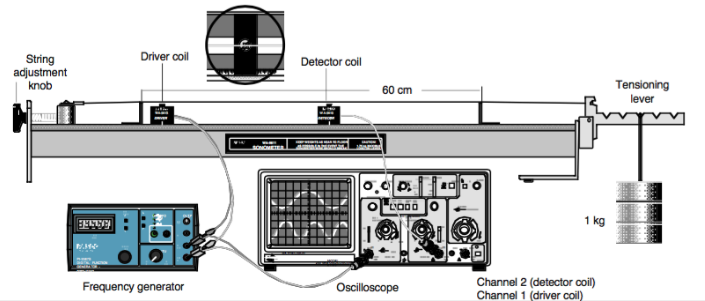
\includegraphics[width=\linewidth]{wave app.png}
    \caption{\centering Illustration of the apparatus setup \protect\cite{UCDwave}.}
    \label{fig:appillust}
\end{figure}

\begin{minipage}{.31\textwidth}
    \captionsetup{hypcap=false}
    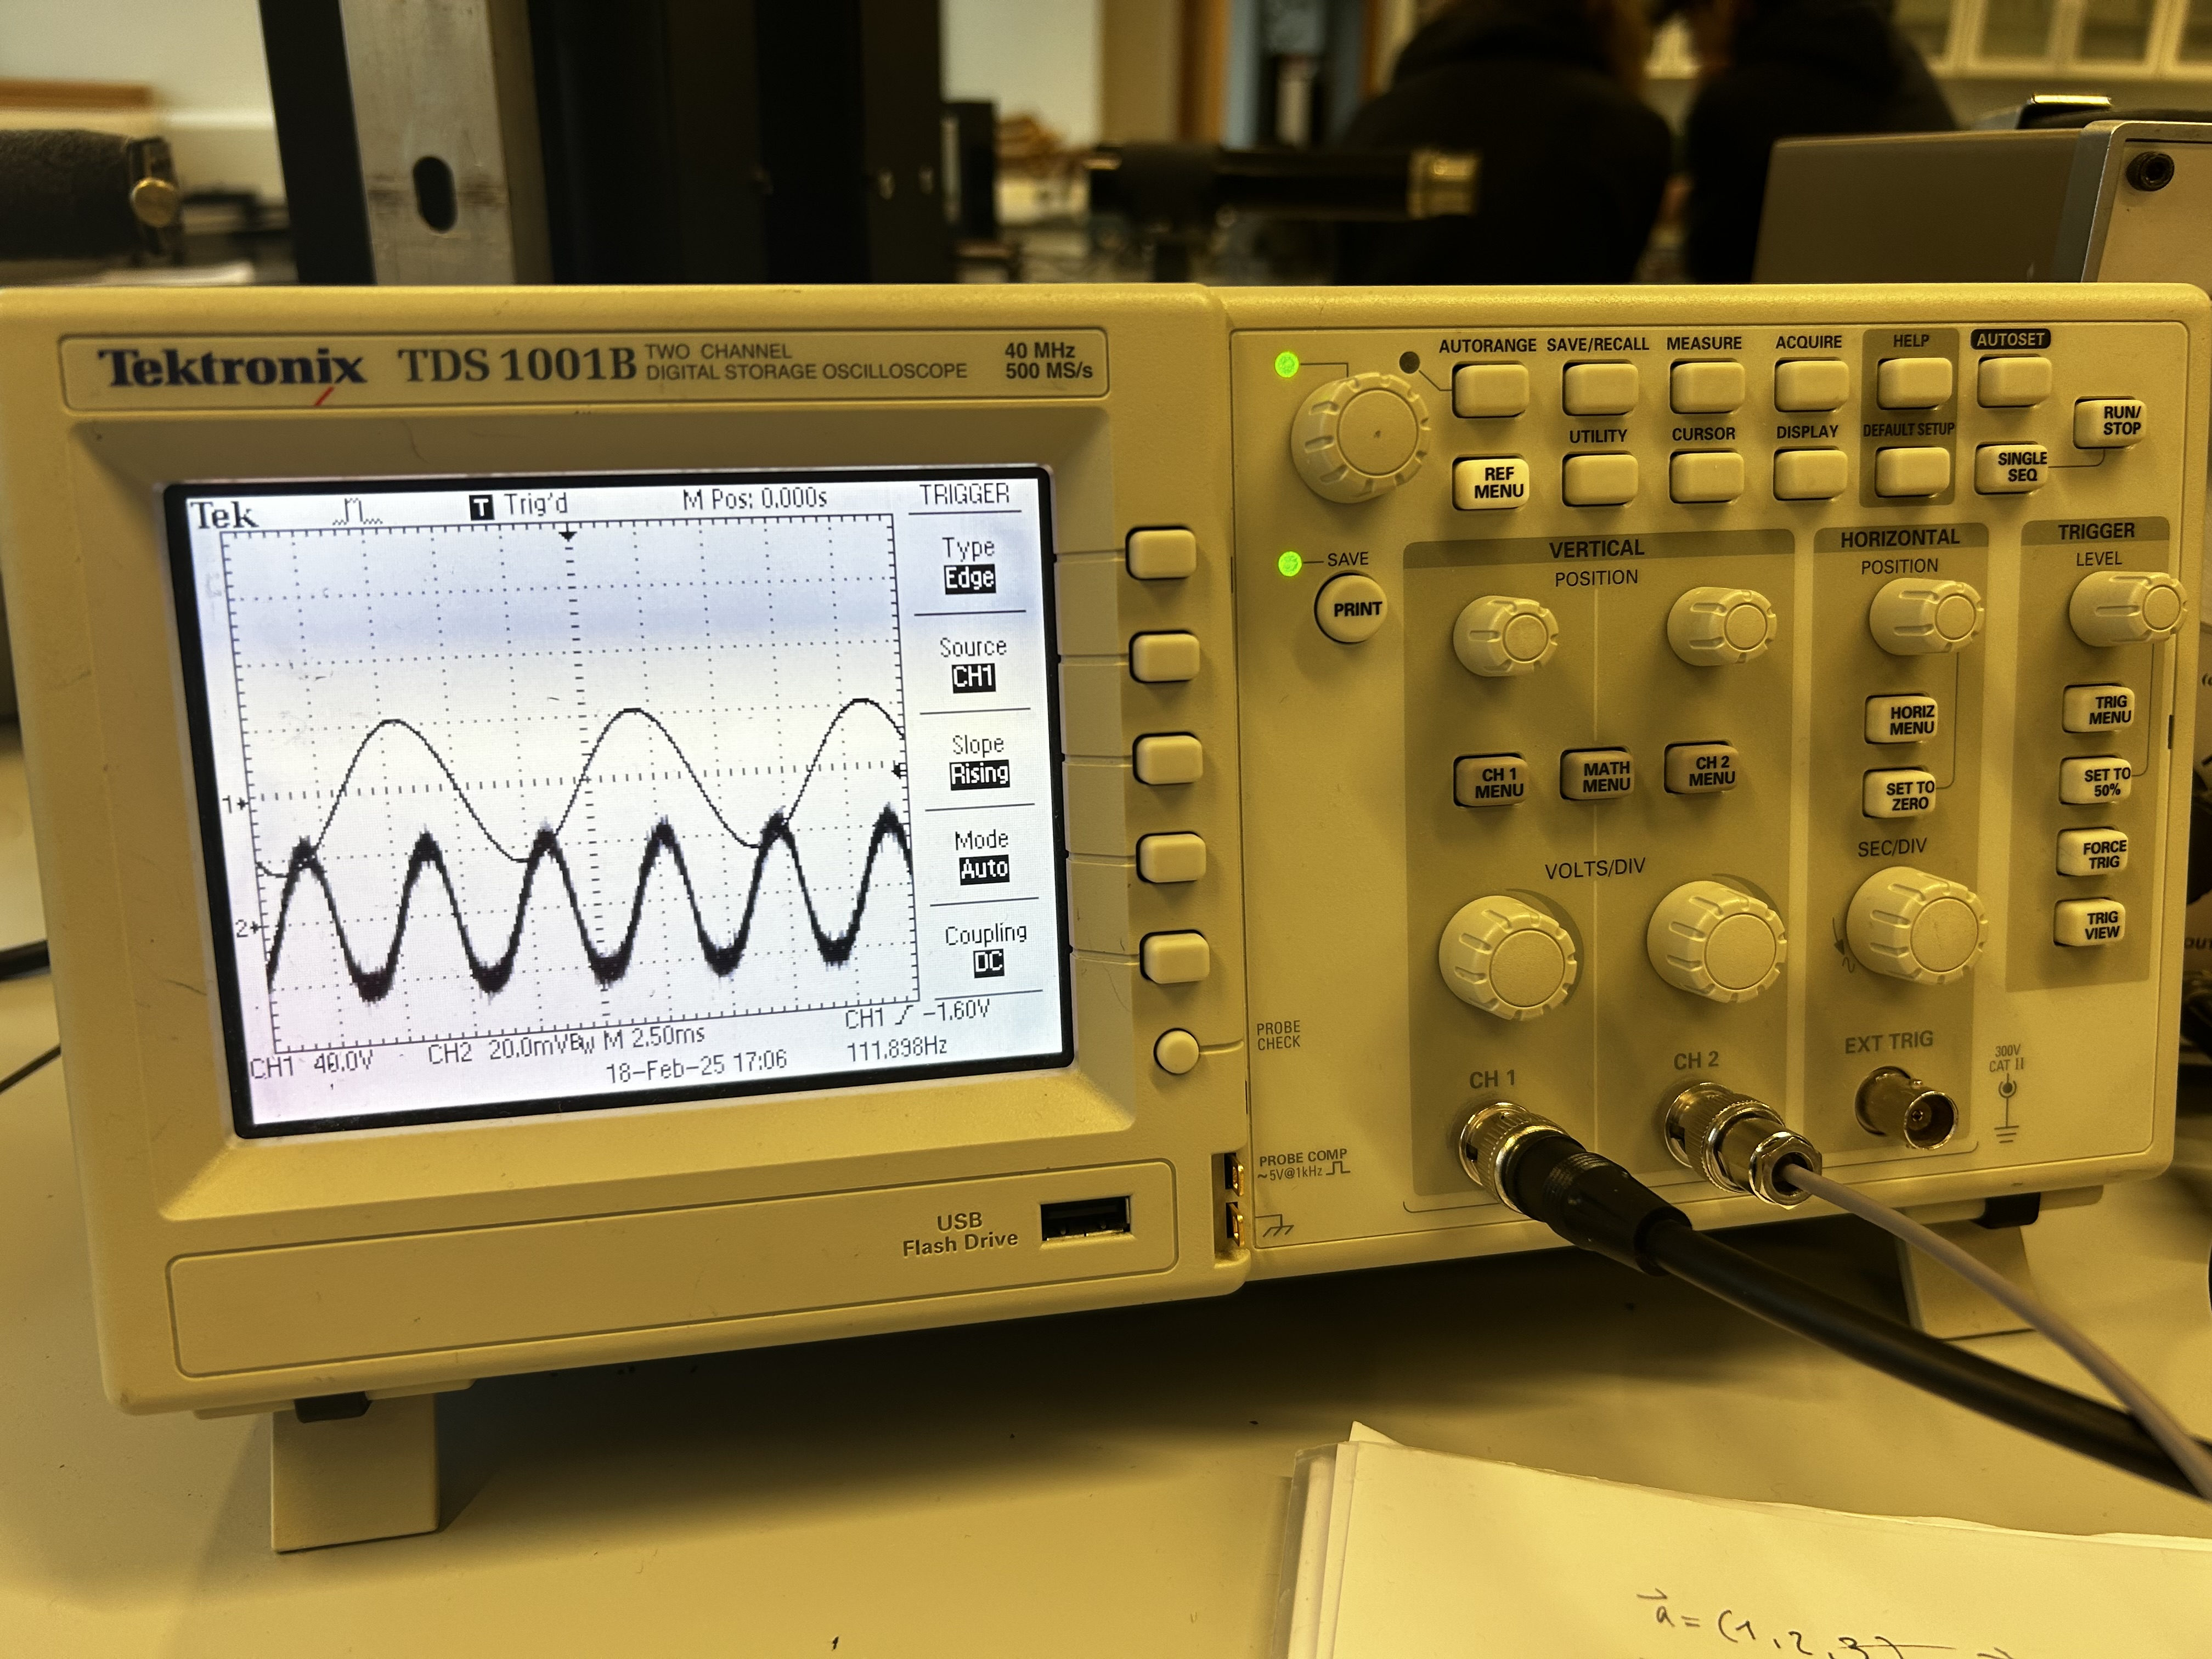
\includegraphics[width=\linewidth]{wave exp 1.jpeg}
    \captionof{figure}{\centering Image of the oscilloscope.}
    \label{fig:oscil}
\end{minipage}
\hfill
\begin{minipage}{.31\textwidth}
    \captionsetup{hypcap=false}
    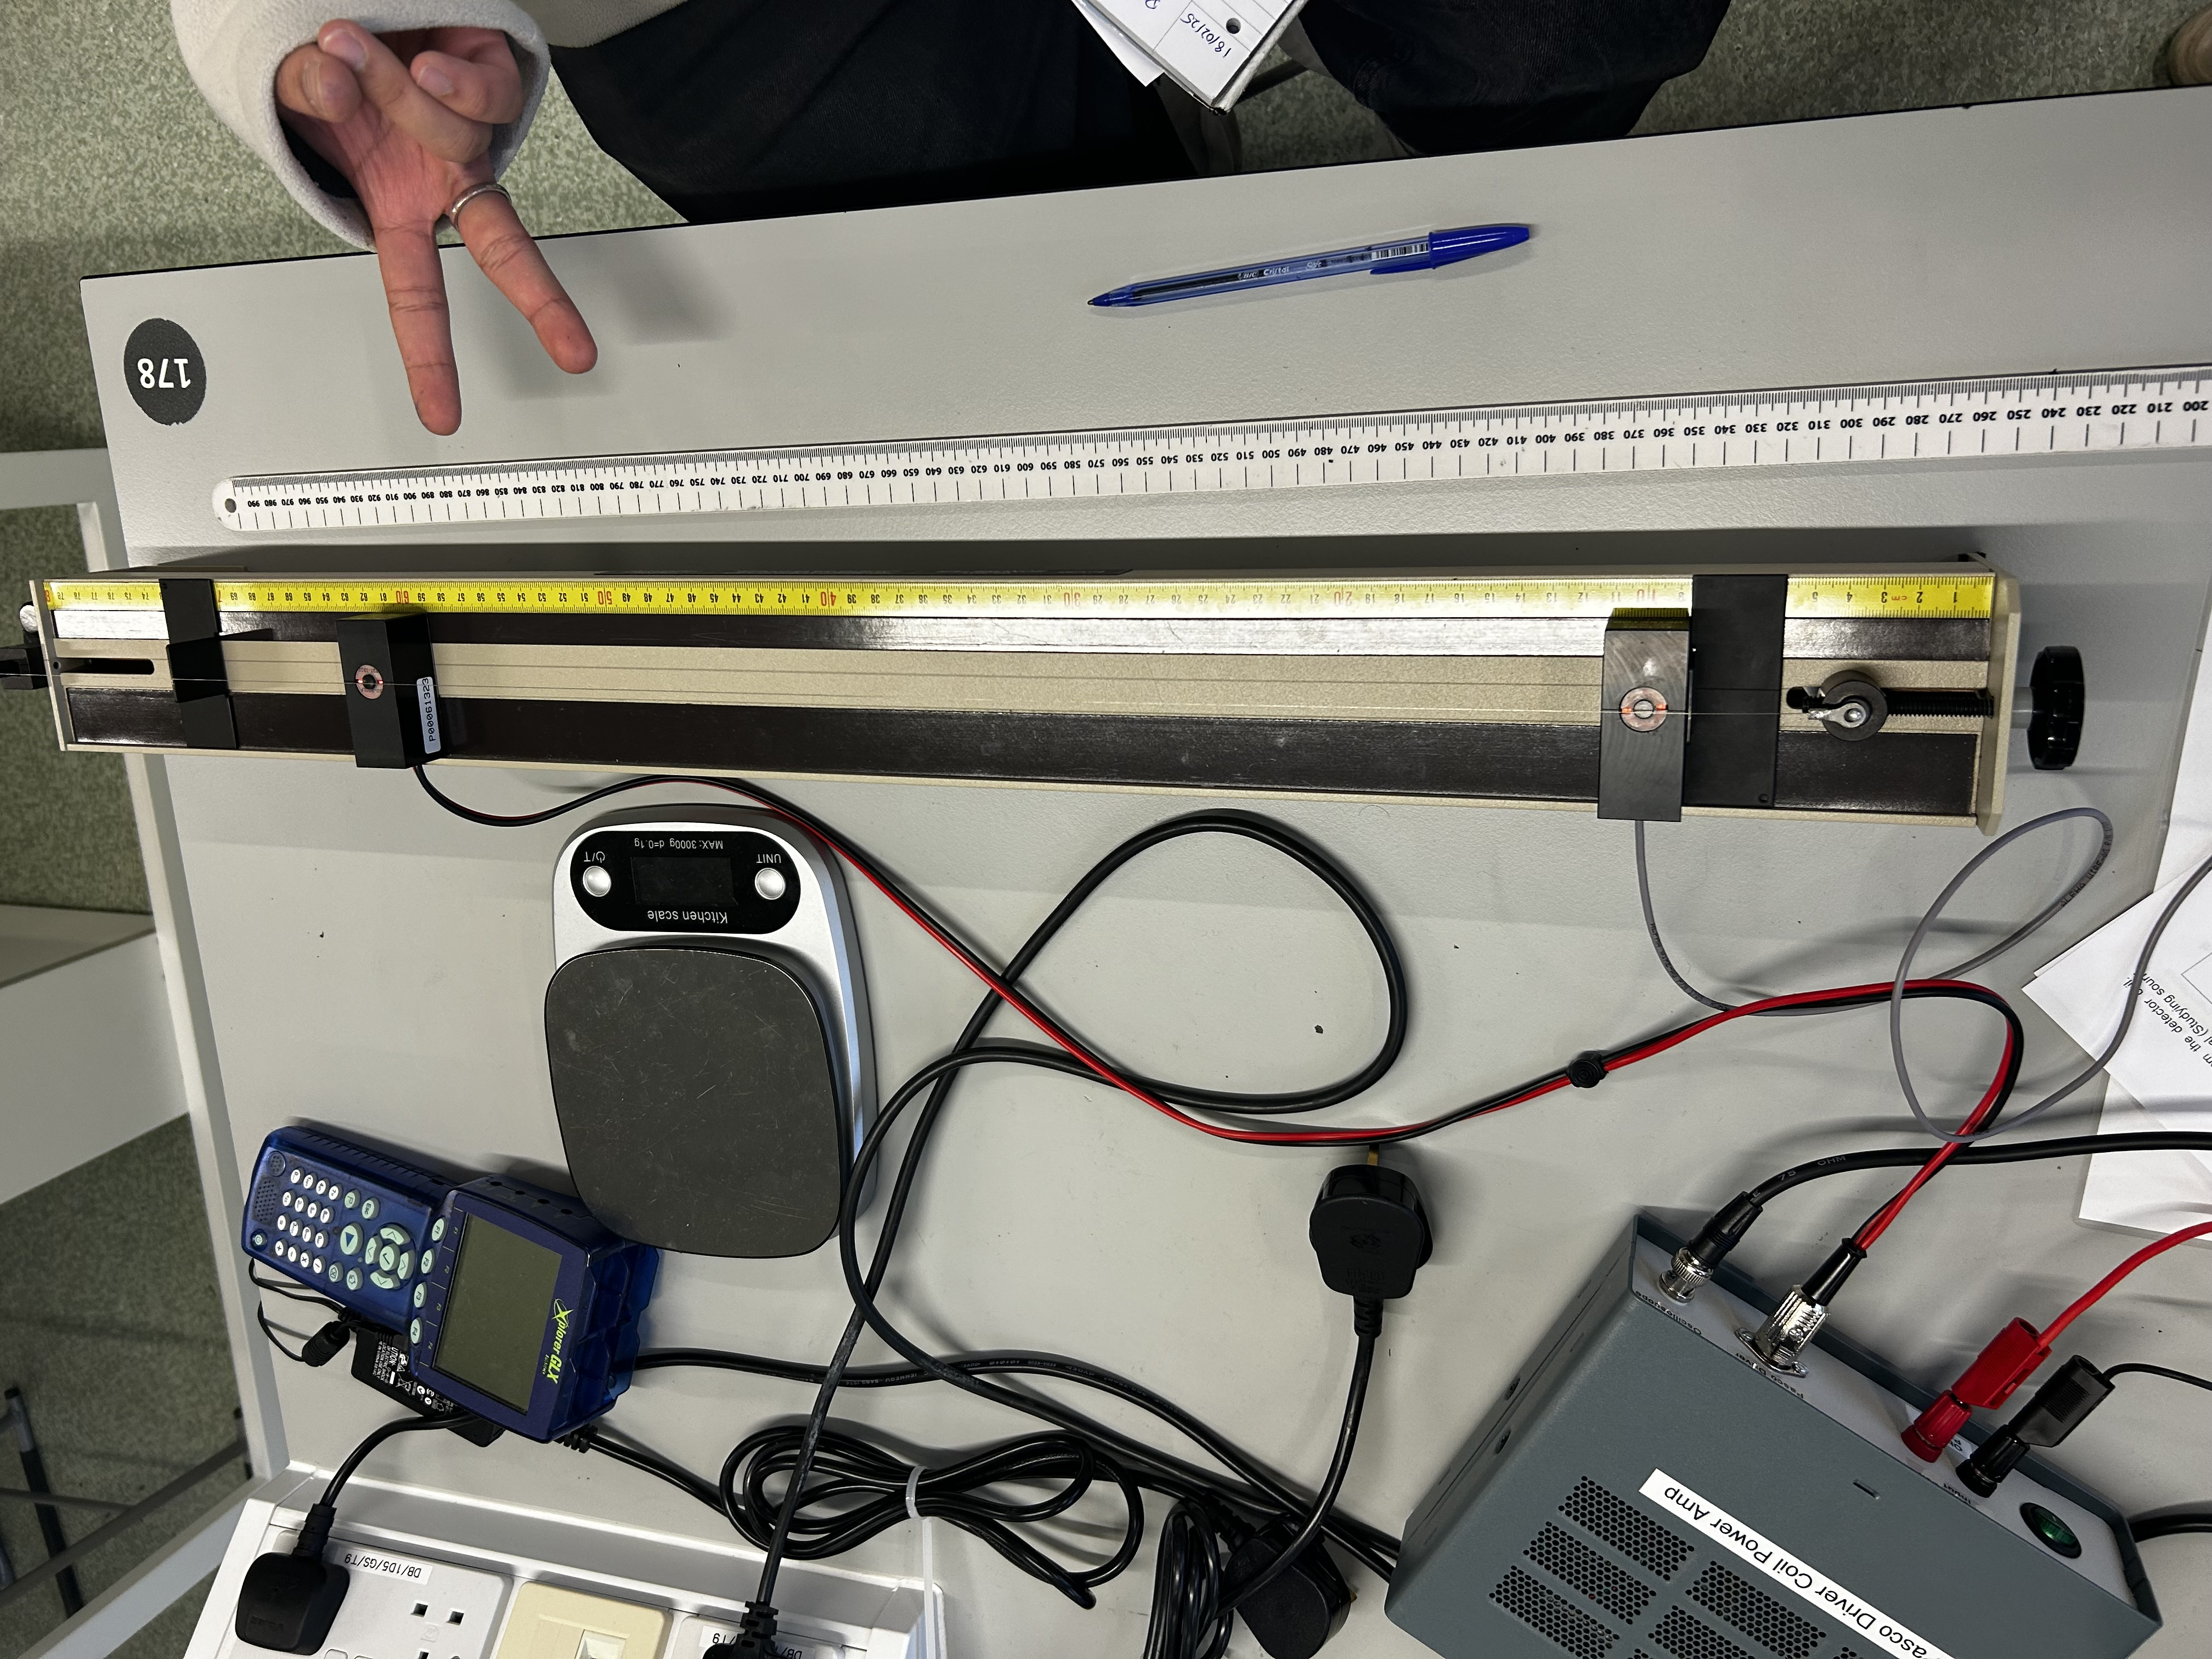
\includegraphics[width=\linewidth, angle=180]{wave exp 2.jpeg}
    \captionof{figure}{\centering Image of the experimental setup.}
    \label{fig:exp}
\end{minipage}
\hfill
\begin{minipage}{.31\textwidth}
    \captionsetup{hypcap=false}
    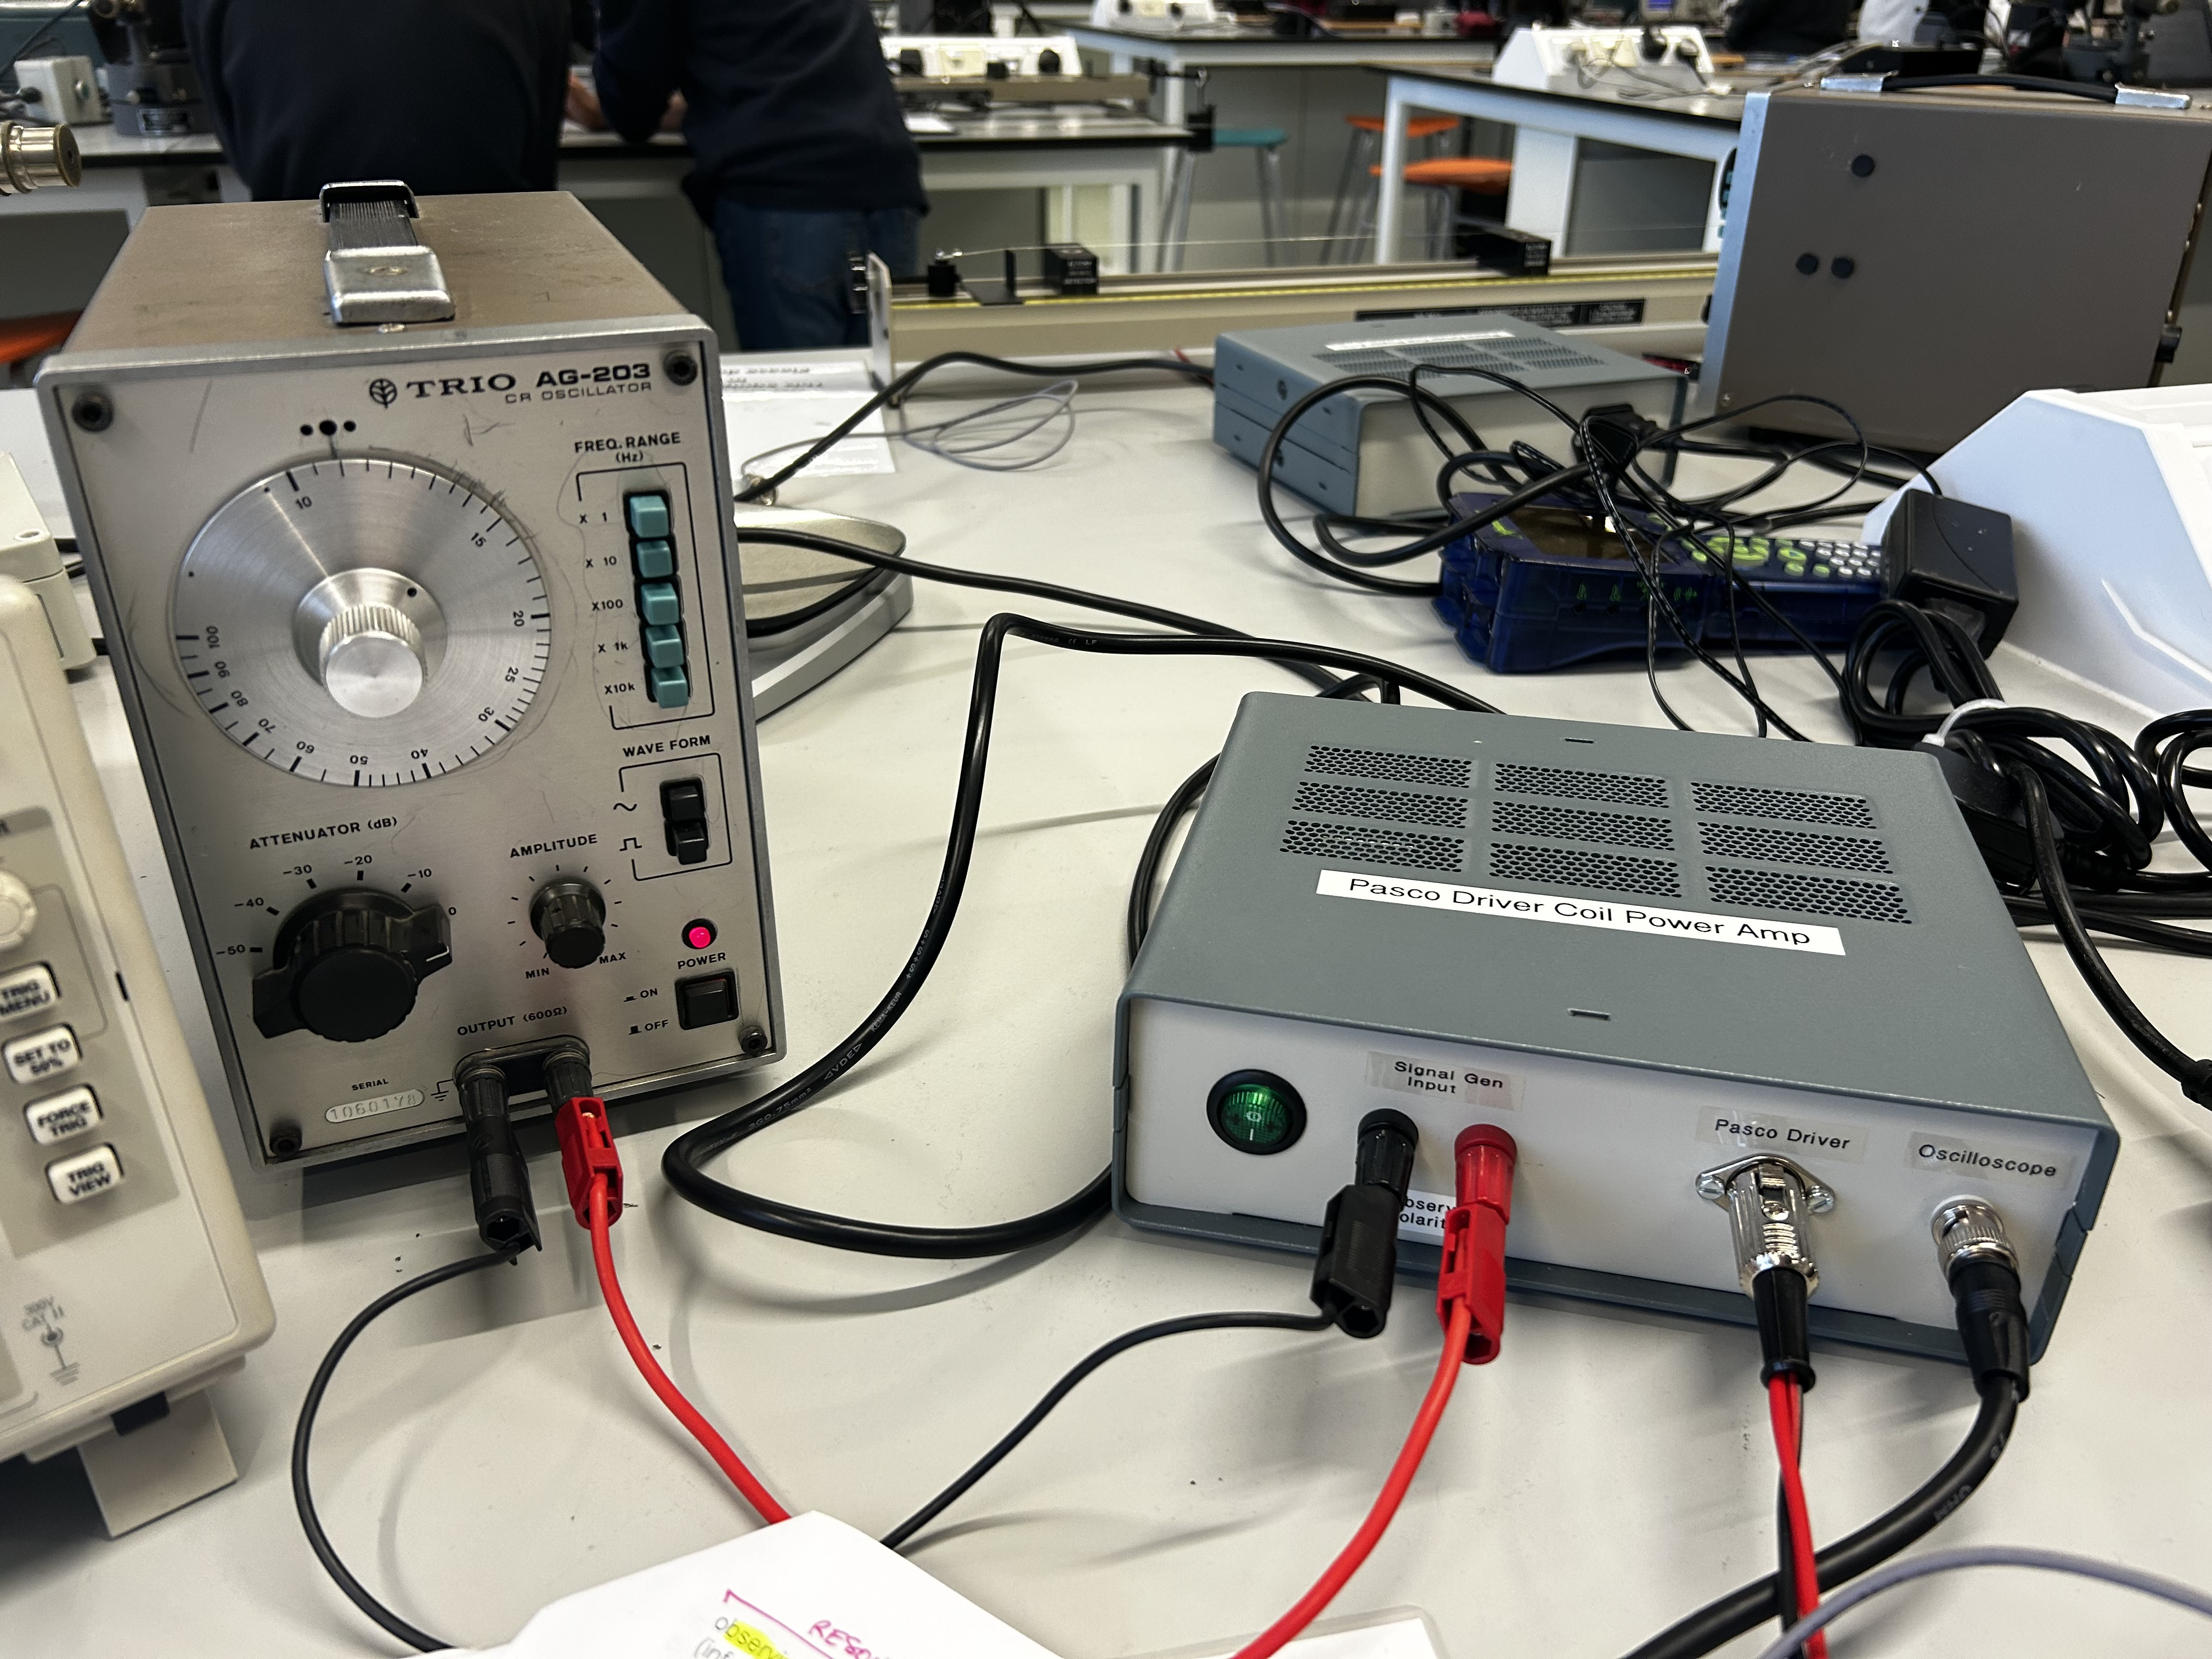
\includegraphics[width=\linewidth]{wave exp 3.jpeg}
    \captionof{figure}{\centering Image of the oscillator.}
    \label{fig:box}
\end{minipage}

The tension in the string was measured using the below formula for both parts of the experiment:

\vspace{-1.5ex}
\begin{gather}
    T = sMgz
\end{gather}

Where \textbf{s} is the slot number, \textbf{M} is the mass, \textbf{g} is the acceleration due to gravity, and \textbf{z} was the constant $0.26$.
From there, the lowest frequency at which resonance (maximum vibrations occur) was found for each varied value and recorded to be plotted in a graph.

\subsection{Varying Length Method}

For this section of the experiment the length of the string that oscillates was adjusted with teh driver and detector coil bridges as seen in figure \ref{fig:appillust}.
The length of this string was then measured with the meter stick on the apparatus, as seen in figure \ref{fig:exp}.

The slot of the weight on the tensioning level was set and left at 3, removing it as a variable for this section of the experiment.

\subsection{Varying Tension Method}

For this section of the experiment the tension of the string was varied by adjusting the slot at which the weight hung from as seen in figure \ref{fig:appillust}.

The length of the string was kept at 60 cm to remove it as a variable from the calculations.

\section{Results and Calculations} \label{sec:3}

\subsection{Application of Theory Questions}

\textit{\textbf{Q1.} A string on a guitar is 1 m long and held under a tension of 100 N. If the string has a mass of 10 g, what is the velocity of a wave on the string?}

\vspace{-1.5ex}
\begin{gather*}
    \mu = \frac{m}{L} = \frac{10 \times 10^{-3}}{1} = 10 \times 10^{-3} \text{ kg m}^{-1}
\end{gather*}
\begin{gather*}
    \implies \quad v = \sqrt{\frac{T}{\mu}} = \sqrt{\frac{100}{10 \times 10^{-3}}} = \mathbf{100 \textbf{ m s}^{-1}}
\end{gather*}

\textit{\textbf{Q2.} If a wave with a frequency of 50 Hz is sent into the string, what will its wavelength be?}

\vspace{-1.5ex}
\begin{gather*}
    v = f \lambda \quad \implies \quad \lambda = \frac{v}{f} = \frac{100}{50} = \mathbf{2} \textbf{m}
\end{gather*}

\textit{\textbf{Q3.} What is the lowest resonant frequency (the fundamental) of the bass guitar string referred to above?}

\vspace{-1.5ex}
\begin{gather*}
    \lambda_{1} = \frac{2(1)}{1} = \mathbf{2} \textbf{m} \qquad\qquad n = 1 \:\: (fundamental) 
\end{gather*}

\textit{\textbf{Q4.} What happens if a wave with a frequency which is the same as the resonant frequency enters the string?}

The string will resonate in its first (fundamental) harmonic (see §\ref{sec:1.2.2}).

\textit{\textbf{Q5.} What happens if a wave with a frequency which is different to the resonant frequency enters the string?}

No standing wave will be formed, and thus the reflection of the wave will result in little to no resonance in the string. No nodes or anti-nodes will be formed or visible as the energy is dissipated rather than amplified.

\subsection{Varying Length}

\begin{minipage}{0.45\textwidth}
    \captionsetup{hypcap=false}
\begin{table}[H]
    \centering
    \begin{tabular}{|c|c|c|}
    \hline
    \textbf{L (cm)} & \textbf{$\mathbf{F_{res}}$ (Hz)} & \textbf{1/L (cm$\mathbf{^{-1}}$)} \\ \hline
    50 & 111.888 & 0.020 \\ \hline
    45 & 111.973 & 0.022 \\ \hline
    40 & 112.033 & 0.025 \\ \hline
    35 & 112.002 & 0.029 \\ \hline
    30 & 112.004 & 0.033 \\ \hline
    25 & 112.129 & 0.040 \\ \hline
    20 & 112.075 & 0.050 \\ \hline
    15 & 112.060 & 0.067 \\ \hline
    \end{tabular}
    \caption{\centering Table of the data gathered for the resonant frequency while varying the lenght of the string.}
    \label{tab:1}
\end{table}
\end{minipage}
\hfill
\begin{minipage}{.5\textwidth}
    \captionsetup{hypcap=false}
    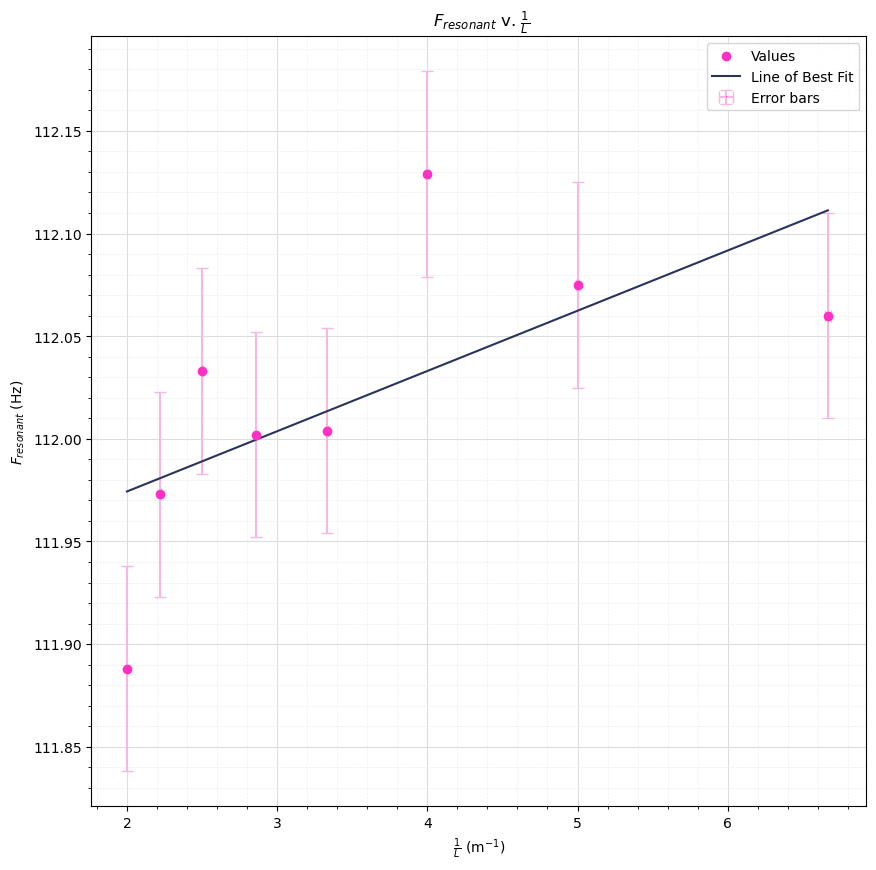
\includegraphics[width=\linewidth]{waves length graph.png}
    \captionof{figure}{\centering Graph of the data found from table \ref{tab:1}.}
    \label{fig:lengthgraph}
\end{minipage}

\subsection{Varying Tension}

\begin{minipage}{.45\textwidth}
    \captionsetup{hypcap=false}
\begin{table}[H]
    \centering
    \begin{tabular}{|c|c|c|}
    \hline
    \textbf{T (N)} & \textbf{$\mathbf{F_{res}}$ (Hz)} & \textbf{$\mathbf{F_{res}^2}$ (s$\mathbf{^{-2}}$)} \\ \hline
    0.2592 & 62.676  & 3 928.281  \\ \hline
    0.5184 & 85.081  & 7 238.777  \\ \hline
    0.7776 & 104.979 & 11 020.590 \\ \hline
    1.0369 & 120.806 & 14 594.090 \\ \hline
    1.2961 & 133.430 & 17 803.565 \\ \hline
    \end{tabular}
    \caption{\centering Table of the data gathered for the resonant frequency while varying the tension on the string.}
    \label{tab:2}
\end{table}
\end{minipage}
\hfill
\begin{minipage}{.5\textwidth}
    \captionsetup{hypcap=false}
    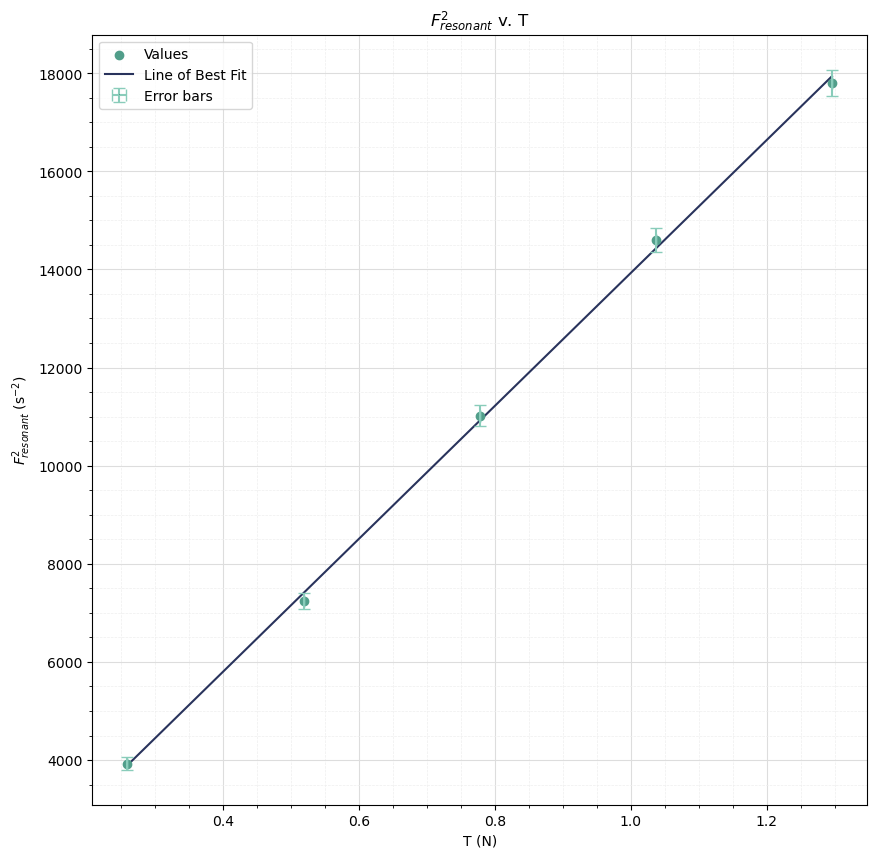
\includegraphics[width=\linewidth]{waves tension graph.png}
    \captionof{figure}{\centering Graph of the data found from table \ref{tab:2}.}
    \label{fig:tensiongraph}
\end{minipage}

\newpage

\section{Conclusion} \label{sec:4}



\section{Applications of Resonant Frequency}

\subsection{Electrical Resonance}

Information and citations sourced directly from one of my previous lab reports as information applies here \cite{meUCDlcr}.

\subsubsection{Radios Transmissions and TV Broadcasts}

Radios make use of frequency resonance to tune into broadcasts operating at specific frequencies on analogue radios, which can be heard once the the elements of the resonant circuit are in equilibrium
\cite{radio}. 
If the peak of the frequency band is too sharp some information, like high frequencies, may be lost
\cite{UCDlcr}.

\subsubsection{Environmental Monitoring}

Resonant circuits can be used in \textbf{temperature monitoring}, in which variations in \break temperature effect changes in the inductance and capacitance sensor, thereby changing the resonant frequency.
The same principle is used in \textbf{humidity monitoring}, where increases in permittivity and conductivity (proportional to humidity) leads to decreases in sensor resonant 
frequency.
This can then be expanded upon to determine \textbf{complex permittivity}, and in turn \textbf{biological growth monitoring} by measuring the changes in complex permittivity.
As humidity and temperature are bases for bacterial culture growth, changes in the Q-factor and resonant frequency can be used to monitor these developments.
Additionally, changes in the resonant frequency can also be used for \textbf{pressure monitoring} as increases in pressure are directly proportional to changes in temperature ($P \propto T$) (and, in turn, humidity).
More information with graphical and mathematical justification can be found at source \cite{ONG200133}.

\newpage

%%%%%%%%%%%%%%%%%%%%%%%%%%%%%%%%%%%

\bibliographystyle{IEEEtran}
\bibliography{References} \label{sec:ref}

\vspace{1.5cm}

\listoffigures

\listoftables

\section*{Appendix} \label{sec:A}
\addcontentsline{toc}{section}{Appendix}

\subsection*{Tables}
\addcontentsline{toc}{subsection}{Tables}



\subsection*{Graphs}
\addcontentsline{toc}{subsection}{Graphs}



\subsection*{Code}
\addcontentsline{toc}{subsection}{Code}

%

\begin{minipage}{\linewidth}
\captionsetup{hypcap=false}

\begin{mintedbox}
\begin{minted}[fontsize=\small, breaklines, baselinestretch=1.2, xleftmargin=0.5cm]{python}

import numpy as np

\end{minted}
\end{mintedbox}

\end{minipage}



\end{document}